\chapter{Special protection schemes}
\label{ch:SPS}

This chapter is based on the following publication:
\begin{itemize}
    \item \fullcite{LambdaMu2022}
\end{itemize}

As discussed previously, dynamic stability issues are becoming prevalent in many power systems due to various causes such as market liberalisation, intermittent energy sources, increase of static limits (thanks to better conductors and dynamic line rating), etc. There are three main general solutions to mitigate dynamic issues:

\begin{itemize}
    \item Installation of new transmission infrastructure and upgrade of existing installations (lines, transformers, etc.): this solution is potentially the most effective but it has the drawback of high lead times (up to ten years) and costs. Also, due to public and regulatory pressure, TSOs have to give more and more justifications to choose this option.
    \item Redispatching: redispatch actions such as curtailment of renewable generation can also mitigate dynamic issues. However, these actions drive the system away from the economical optimum. These actions can be judged cost-prohibitive as they have to be performed each time a (plausible) disturbance threatens the stability of the system while the probability of the disturbance actually occurring can be very low. (Line switching is a low-cost redispatching action, but it cannot alleviate all issues on its own.)
    \item Special protection schemes (SPSs): SPSs are schemes that automatically perform corrective actions upon detection of a disturbance. These schemes lead to lower operating costs since corrective actions only have to be performed after a disturbance actually occurs. They are also significantly less expensive and quicker to install than transmission infrastructure. SPSs have to act quickly to be effective, usually in dozens of milliseconds to a few seconds. Possible actions that can be taken by a SPS include: generation rejection, turbine fast valving, braking resistor, fast unit start-up, governor setpoint change, load shedding, shunt switching, HVDC fast power change, on-load tap changer (OLTC) blocking, quick increase of synchronous condenser and FACTS voltage setpoint, and system splitting~\cite{CigreDefensePlan}.
\end{itemize}

Case-specific solutions (e.g. fast frequency response to mitigate frequency instability, OLTC blocking to mitigate voltage instability, etc.) are also important but are too numerous to be discussed here. This chapter focuses on SPSs and in particular how to consider them in a probabilistic dynamic security assessment. In particular, section~\ref{sec:SPSreliability} discusses reliability considerations regarding SPSs and section~\ref{sec:SPS-ICT} discusses the communication infrastructure necessary to use SPSs as well as potential threats linked to communications. Finally, section~\ref{sec:SPSperspectives} concludes with perspectives of future work regarding SPSs.

In the literature, various definitions of SPSs exist. In this thesis, the following definitions are used. A system integrity protection scheme (SIPS) is a protection scheme whose primary objective is to protect the integrity of the whole power system. This contrasts with classical protection schemes whose primary objective is to protect a given element against unacceptable conditions (including sustained faults). A SPS is any SIPS that is not a local under-frequency load shedding (UFLS) or under-voltage load shedding (UVLS) scheme. The term defence plan is also used in the literature. SIPSs are often the main elements of a defence plan, although other (slower) mitigation measures are also included~\cite{CigreDefensePlan, ENTSOEdefencePlan}. This term is however not used in the remaining of this thesis.

\section{Reliability considerations}
\label{sec:SPSreliability}

The integration of SPSs is usually done in two phases. In the first phase, the TSO designs a SPS to mitigate a specific problem in the system. This SPS requires data from only a few buses to detect this specific problem and has a small set of possible actions. In this phase, the SPS usually has a dedicated ICT infrastructure~\cite{BelgiumSPS}. In the second phase, the TSO starts to rely on SPSs to mitigate various issues. In this case, a more scalable design consists of a centralised Control Centre (CC) that has access to measurements from most buses in the system. Then, a dedicated ICT infrastructure makes less sense. The SPS thus uses the existing ICT infrastructure used for traditional operations~\cite{GeorgiaSPS, UruguaySPS}. Beyond scalability, an advantage of the second type of SPS is that they can make use of classical state estimation algorithms to compute the most likely state of the whole system even with partial information.

The reliability of the two types of SPSs has to be evaluated with different methodologies. The first type of SPS usually has a dedicated communication infrastructure and requires a limited number of remote measurements. The reliability of this kind of SPS can thus be modelled using standard reliability analysis such as reliability block diagrams and fault trees. An example of such an approach can be found in~\cite{SPSreliabilityThesis} and the references therein. It should however be noted that due to their relative low cost and critical nature, those SPSs are usually designed with a very high level of reliability (both selectivity and dependability). For example, the SPS presented in~\cite{BelgiumSPS} determines the state of each line end using a 2-out-of-4 voting scheme. It also has two redundant communication infrastructures, and it has been extensively tested prior to installation. It might thus not be necessary to include the possible misoperation (nor unwanted nor missing operations) in a probabilistic security assessment. It can be considered in a more possibilistic approach, but this is out of scope of this thesis.

The reliability analysis of the second type of SPS can be decomposed into three parts: state estimation, communication and control actions. Estimating the state of the system requires to have a sufficiently large (and diverse) set of measurements. Observability analysis can be used to determine if a given set is appropriate. It should be noted that the (relatively recent) large-scale installation of phasor-measurement units (PMUs) implies that the random loss of a few measurements should have very limited impact on the state estimation performed by the SPS. It is thus mostly inadequate performance of the communication infrastructure that can potentially lead to poor state estimation. The performance of the communication infrastructure is discussed in section~\ref{sec:SPS-ICT}. Once the SPS has evaluated the state of the system, identified a disturbance and successfully sent a control action to one or several actuators, those actuators have to actually implement the corrective action. The performance of the actuators can again be evaluated using standard reliability methods (fault trees, etc.).

\section{ICT infrastructure}
\label{sec:SPS-ICT}

The first type of SPS has a very simple communication infrastructure and is thus no longer considered in the remaining of this chapter. Most of the literature on (the second type of) SPSs simulate the ICT infrastructure by simulating it with network\footnote{In this thesis, network is short for communication network, and grid is short for electrical grid.} simulators such as ns-3, OMNeT++ or OPNET~\cite{SPS-Ciapessoni}. Some even use co-simulations, i.e. interface power system and network simulators and make them run together~\cite{SPS-MingNi, GECOtestcase}. Co-simulation is discussed in more details in appendix~\ref{ch:CYPRESS}. In this thesis however, it is preferred to use basic queuing theory. This approach allows to have an analytical formulation for the delays in the ICT system. It thus allows to have a better understanding of the system and to explore the impact of disturbances more easily.

So, queuing theory is introduced and used to size the ICT infrastructure in section~\ref{sec:ICTsizing}. Then, it is used to study the impact of failures in section~\ref{sec:ICTfailure}. A simple method to monitor the communication performance in real-time is then proposed in section~\ref{sec:ICTmonitoring}. Finally, the impact of different types of cyber-attacks is discussed in section~\ref{sec:ICTtrafficAttack}.


\subsection{Infrastructure sizing}
\label{sec:ICTsizing}

The test case considered in this section is the Roy Billinton test system (shown in Fig.~\ref{fig:RBTS-phys}) equipped with a centralised SPS. The SPS consists in PMUs that are installed at each bus and send measurements (voltage, current, frequency and possible breaker status) to a CC located near bus 3. The ICT infrastructure is shown in Fig.~\ref{fig:RBTS-cyber}. In real networks, phasor data concentrators (PDCs) are placed between the PMUs and the CC to aggregate the PMU traffic. This is is not the case here due to the small size of the system considered. The methods presented below can however easily be adapted to consider those PDCs.

It is necessary to have a communication infrastructure to link the PMUs to the CC. TSOs can either have their own infrastructure, this is e.g. the case in the UK~\cite[p110]{bookUK_OPGW} and in Germany~\cite[p42]{ThesisInspire} where optical ground wires (OPGWs) are installed on top of most transmission lines, or rent it from an Internet service provider (ISP). In the second case, the design of the infrastructure is outsourced to the ISP\footnote{There is a tendency of operators of geographically-extended systems (e.g. railroads) to install fibre optic cables in parallel to their infrastructure and to sell them to ISPs. Part of the capacity of the cables is then rented back to the utility. There are two main causes to this trend. First, the bandwidth of modern cables often vastly exceeds the needs of utilities. Second, ISPs have more experience in managing communication infrastructures. A concern that this introduces is that critical communication infrastructures (electricity, railroad, etc.) get connected to the global internet. However, it has been shown many times that and ``air gap" is not an effective cyber-security measure.}. The focus is thus placed on the first case. However, ISPs use a similar methodology to what is described below. Also, for the sake of simplicity, it is assumed that a single OPGW is installed in parallel to every transmission line (including the double lines).

\begin{figure}
     \centering
     \begin{subfigure}[b]{0.45\textwidth}
         \centering
         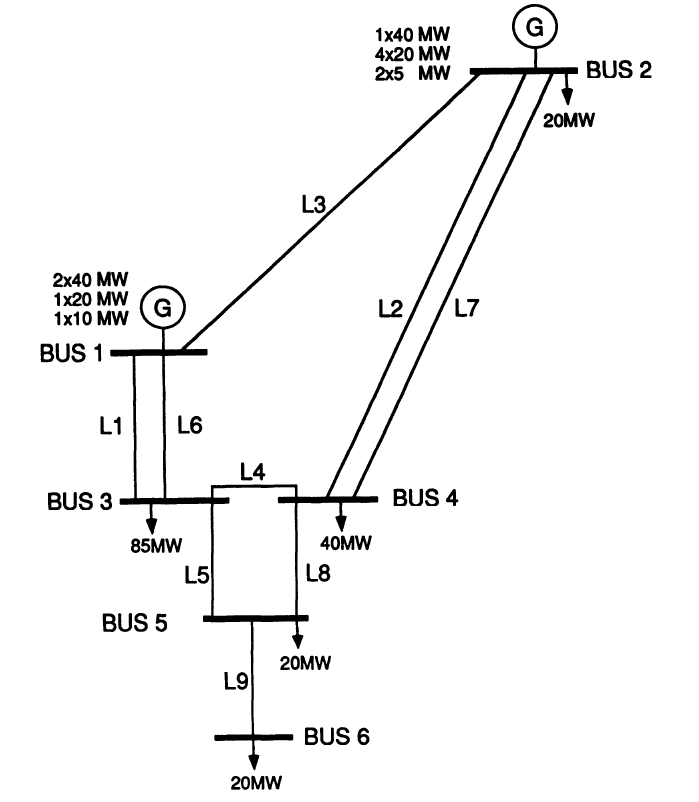
\includegraphics[width=\linewidth]{Figs/RBTS.png}
         \caption{Physical part. Adapted from~\cite{rbts}}
         \label{fig:RBTS-phys}
     \end{subfigure}
     \hfill
     \begin{subfigure}[b]{0.45\textwidth}
         \centering
         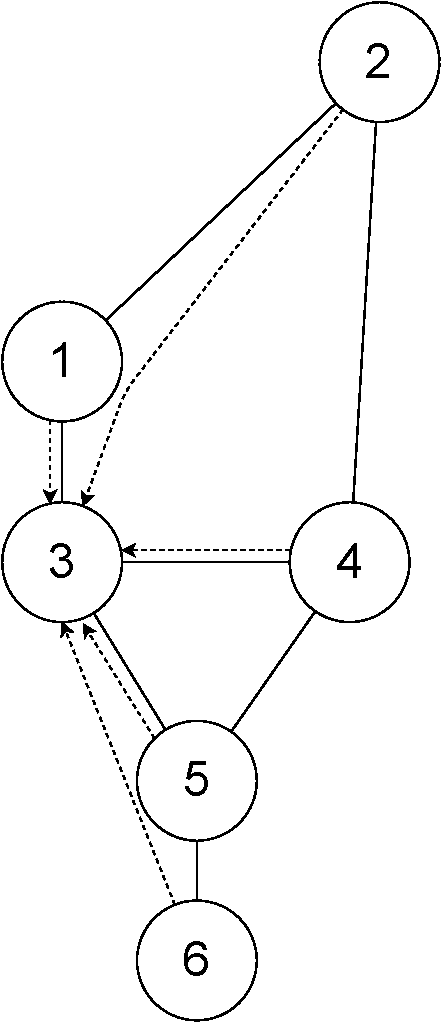
\includegraphics[width=0.5\linewidth]{Figs/RBTS_com.pdf}
         \caption{Communication infrastructure. Plain lines represent communication links, and dashed arrows represent PMU traffic flows in normal operation}
         \label{fig:RBTS-cyber}
     \end{subfigure}
\caption{Cyber-physical Roy Billinton test system (RBTS)}
\label{fig:RBTS}
\end{figure}

TSOs usually only use a fraction of the bandwidth provided by the OPGWs. They thus often choose to rent part of this bandwidth to ISPs~\cite[p110]{bookUK_OPGW}. The traffic used for the SPS should however not be in competition with the ISPs' traffic. This is achieved using quality of service (QoS) mechanisms such as weighted fair queuing. These mechanisms allow to guarantee a given amount of bandwidth for the SPS. Below, queuing theory is used to determine the minimum bandwidth to reserve for the SPS to stay under a maximum delay.

The most common assumption in communication network traffic engineering is to consider that the distribution of arrivals is Poissonian~\cite{trafficBook}. In other words, it means that packets arrive with a constant mean rate and independently of the time elapsed since the last event. This assumption is very often valid in ISP networks due to the large number of independent inbound traffic sources\footnote{The validity of this hypothesis in the communication network of an SPS is discussed later in this section.}. Then, traffic load (or traffic intensity) of an element (router, firewall, etc.) is defined as:
%
\begin{equation}
\rho = \lambda/\mu
\end{equation}
%
where \(\lambda\) is the arrival rate of packets in the element [packets/s], and \(\mu\) is the processing rate of the element [packets/s]. Then, from the Poisson assumption, a well-known result from queuing theory~\cite{trafficBook} is that the average number of packets in the queue of the element is given by\footnote{Assuming a steady-state system, infinite buffer size, and \(\rho \leq 1\)}:
%
\begin{equation}
N = \frac{\rho}{1-\rho}
\end{equation}
%
We can then use Little's law~\cite{littleLaw} that states that the average queuing time \(t_q\) [s] spent by a packet in a system is given by:
%
\begin{equation}
\label{eq:little}
t_q = N/\lambda
\end{equation}
%
(Little's law is valid for any stationary system, e.g. a single queue or a complex network.) It is also interesting to decompose \(t_q\) into the waiting time \(t_w\) and the processing time \(t_s = \frac{1}{\mu}\). For this, one can simply observe that when a packet arrives in a queue, it must wait for the average \(N\) packets already present to be processed. So,
%
\begin{equation}
\label{eq:t_w}
t_w = N t_s
\end{equation}
%
Eq.~(\ref{eq:little}) and~(\ref{eq:t_w}) imply that,
%
\begin{equation}
t_w = \frac{\rho}{1-\rho} t_s
\end{equation}
%
and,
%
\begin{equation}
\label{eq:final}
t_q = \frac{1}{1-\rho} t_s
\end{equation}
%
Eq.~(\ref{eq:final}) is plotted in Fig~\ref{fig:queuing}. This figure illustrates clearly the impact of congestion on delays. This figure shows that, in order to limit the waiting delay (and its derivative with respect to \(\rho\)), the network should be operated such that \(\rho\) is lower than 0.7 or even 0.5.

\begin{figure}
\centering
\begin{tikzpicture}
\pgfplotsset{width=0.6\linewidth}
        % legend style={font=\footnotesize}}
\begin{axis}[
    xlabel={Traffic intensity},
    ylabel= {\(t_q/t_s\)},
    enlarge x limits=0,
    enlarge y limits=0,
    xmin = 0,
    xmax = 1,
    xtick distance = 0.2,
    ytick distance = 2,
    ymin = 0,
    ymax = 8,
    smooth,
   ]

  \addplot [name path=A, blue, no marks, domain=0:0.95] {1/(1-x)};
  \addplot [name path=B, black, no marks, dashed] {1};
  \addplot[blue, fill opacity=0.2] fill between[of=A and B];

  \addplot [red, no marks, dashed] coordinates {(0, 3.33333333) (0.7, 3.33333333)};
  \addplot [red, no marks, dashed] coordinates {(0.7, 0) (0.7, 3.33333333)};

  \node at (axis cs:0.73,1.1) [anchor=south west, text width=5em, align=right] {Excess overhead induced by queuing};

  \node at (axis cs:0.01,3.2) [anchor=north west] {Zone of normal operation};

\end{axis}
\end{tikzpicture}
\caption{Communication delays as a function of congestion}
\label{fig:queuing}
\end{figure}

This methodology is now illustrated on the RBTS. For this, it is assumed that each PMU generates 120~kbps of traffic (packets of 300 bytes~\cite{StandardC37-118-2} sent at 50~Hz), that 300~kbps is reserved in each link for the SPS, and that packets are routed to the shortest path as shown in Fig.~\ref{fig:RBTS-cyber}. Also, the processing time of routers is assumed to be limited by the bandwidth of links, i.e. is equal to the packet size divided by the bandwidth, so 8~ms. The traffic in each link is simply the sum of all traffics going through this link\footnote{For routers where multiple PMU influxes are merged, a Poisson distribution of arrivals can still be assumed thanks to the additivity of the Poisson distribution. Thanks to this additivity property, queuing theory can easily be applied in large networks.}. From this traffic, one can compute the traffic intensity and the average queuing time as done in Table~\ref{tab:delayLink}. Then, the average communication delay between a given PMU and the CC is simply given by the sum of the delays in the path between this PMU and the CC. Those delays are given in Table~\ref{tab:delayPMU}.

\begin{table}
\centering
\caption{Computation of the average time spent by a packet in a given link for a reserved bandwidth of 300~kbps}
\label{tab:delayLink}
\begin{tabular}{|l|l|l|l|l|}
\hline
\multicolumn{1}{|c|}{\textbf{Link}} &
  \multicolumn{1}{c|}{\textbf{Traffic}} &
  \multicolumn{1}{c|}{\textbf{\(\bm{\rho}\)}} &
  \multicolumn{1}{c|}{\textbf{\(\bm{N}\)}} &
  \multicolumn{1}{c|}{\textbf{\(\bm{t_q}\) [ms]}} \\ \hline
2-1 & 120~kbps & 0.4 & 0.67 & 13.3 \\ \hline
1-3 & 240~kbps & 0.8 & 4    & 40   \\ \hline
4-3 & 120~kbps & 0.4 & 0.67 & 13.3 \\ \hline
5-3 & 240~kbps & 0.8 & 4    & 40   \\ \hline
6-5 & 120~kbps & 0.4 & 0.67 & 13.3 \\ \hline
\end{tabular}
\end{table}

\begin{table}
\centering
\caption{Average communication delays between each PMU and the CC}
\label{tab:delayPMU}
\begin{tabular}{|l|l|}
\hline
\multicolumn{1}{|c|}{\textbf{PMU \#}} & \multicolumn{1}{c|}{\textbf{\(\bm{t_q}\) (ms)}} \\ \hline
1                                    & 40                                     \\ \hline
2                                    & 53.3                                   \\ \hline
4                                    & 13.3                                   \\ \hline
5                                    & 40                                     \\ \hline
6                                    & 53.3                                   \\ \hline
\end{tabular}
\end{table}

These delays can be compared with the maximum delay allowable for the SPS's actions. In this case, the SPS protects the system against angle stability issues by disconnecting a 20~MW generator at bus 2 when either line 2, 3 or 7 is lost. In~\cite{LambdaMu2022}, I showed that for this particular system, the generator should be disconnected at most 173~ms after the line loss. To determine the maximum communication delay that satisfy this constraint, the other (constant) delays have to be subtracted from those 173~ms. The processing times in the PMUs and CC is taken as 5 and 10~ms respectively~\cite{SPS-Ciapessoni}. A 20~ms worst-case delay due to the sampling rate of 50~Hz is also considered. The circuit breaker of the generator is supposed to open in 60~ms~\cite{ESOcircuitBreakerDelay}. A constant 8~ms delay is considered for communication between the CC and the generator\footnote{Queuing theory could also be used to compute this delay, however as messages from the CC to the generator travel in the opposite direction as messages from PMUs to the CC, they do not affect each other (assuming full duplex links).}. The propagation delays (1~ms per 200~km for a refractive index of the communication medium of 1.5) are neglected. There is thus 70~ms remaining for the communication delays between the PMUs and the CC. One can then verify than the average delays in Table~\ref{tab:delayPMU} are lower than 70~ms. It is also possible to compute the probability of the delays being lower than 70~ms. This is however more complex, and discussed in traffic engineering textbooks~\cite{trafficBook}.

The computations above have been made assuming a Poisson distribution of arrivals. The PMUs however send packets at a deterministic and constant rate. The developments above are still useful because the merging of several influxes in larger network tends to produce Poisson distributions. Also, the above method will very often lead to conservative results. In this particular case, simulations in ns-3 resulted in communications delays of 8~ms (the processing time in one router) for PMUs 1, 4 and 5, and 16~ms (twice the above value) for PMUs 2 and 6. Finally, due to the small amount of traffic needed by the SPS (and its critical nature), it is inexpensive to have large margins. This is true even for large networks. For example, even if all 2700 substations operated by the french TSO (mostly at 225 and 400~kV level)~\cite{RTEsubstations} send PMU packets (300 bytes~\cite{StandardC37-118-2}) at a sampling rate of 50~Hz, it only results in a total of 360~Mbps\footnote{In the future, the size of the packets might increase slightly due to the transition to IPv6 (20 bytes), additional information regarding substation equipment being included in the PMU traffic (a few dozens of bytes), and longer cryptographic headers (a few dozens of bytes).}.

% If the SPS makes use of demand response, it is also necessary to have a communication infrastructure between the CC (and/or the individual buses) and end-users. Due to high geographical dispersion of end-users, it is completely unrealistic for the TSO to build its own ICT infrastructure for this purpose. The TSO thus has to make service level agreements (SLAs) with distribution system operators (DSOs) or ISPs. The TSO defines the amount of necessary bandwidth and maximum delay, and the DSO or ISP then has to make sure that those constraints are satisfied (e.g. using queuing theory, QoS, etc.).

\subsection{Impact of failure}
\label{sec:ICTfailure}

The impact of cyber failures is studied differently if the ICT infrastructure is owned by the TSO or by an ISP. In the first case, the TSO can simply perform the same analysis as in section~\ref{sec:ICTsizing} but considering that some of the links are failed. For example, after a failure of link 3-4, traffic from the PMU 4 will be redirected through path 4-5, 3-5 which will increase the traffic intensity and queuing delays along this path. A higher bandwidth is thus necessary to stay under the target delay when considering possible failures. Additionally, if simultaneous failures of communication links and power lines are considered (due to a common mode failure), an additional delay has to be considered for the rerouting of the traffic.

In the second case, cyber failures will usually have a lower impact. This is because ICP's networks are usually more meshed than TSO's grids. For example, the core network of BT (formerly British Telecom) consists of 8 inner core nodes that are fully linked to each other, and 12 outer nodes that are each connected to at least 3 core nodes~\cite{BTnetwork}. Also, in this case, it is the ISP and not the TSO that has to make sure the cyber failures have a limited impact on the performance of the ICT infrastructure. The service level agreement (SLA) should define to what level of reliability the ICT performance (i.e. availability and delays) should be guaranteed. Carrier-grade lines are often leased with a reliability level of 99.999\% (i.e. 5 minutes of total downtime per year).

\subsection{Monitoring ICT performance}
\label{sec:ICTmonitoring}

Even if the ICT infrastructure has been appropriately sized (or if this the responsibility has been outsourced to an ISP), it is still useful to monitor its performance and to verify that the delays are under a given bound. Indeed, delays could increase following failures, bugs, attacks, increase of the traffic, etc. When high delays are detected, the SPS should arm schemes that are less time critical (e.g. disconnection additional generators or loads), or send an alarm to the operators such that they take preventive actions (e.g. reduction of the production at bus 2).

Monitoring the communication delays between the PMUs and the CC is direct since the packets sent by PMUs are precisely time-tagged (PMUs' clock are synchronised via GPS). For other communications (e.g. communication with the generator's circuit breaker), this generally is not possible. An alternative is to estimate communication delays from Round Trip Time (RTT) measurements. In other words, when the TSO sends a message to a given recipient, it measures the time that passed between sending the message and receiving the acknowledgement message from the recipient. Assuming a symmetric network, the one-way delay is half the RTT. Since the TSO might not always need to communicate with recipients, it is necessary to use so-called keep-alive messages to have a continuous monitoring of the RTT. RTT measurements are used very often in ICT networks. The RTT-based mechanism used by TCP as defined by the Internet Engineering Task Force standard~\cite{roundTripTime} is presented below for illustration. There are similar mechanisms in other communication protocols such as RTP (Real-Time Protocol).

In TCP, when an application sends a messages, it expects to receive an acknowledgement from the recipient. If it does not receive one, it resends the message. The Retransmission TimeOut (RTO) is defined as the maximum time after which a sender considers that if it did not receive an acknowledgement signal, then its message was lost and must thus be resent. The RTO can thus be seen as an upper bound (with a good probability) of the RTT. As the RTT can vary in time (due to variability of the traffic, seasonal effects, attacks, etc.), a ``smoothed'' RTT is defined. Each time a new measurement R' of the RTT is made, the smoothed RTT is updated according to:
%
\begin{equation}\text{SRTT} = (1-\alpha)\times\text{SRTT} + \alpha\times\text{R'}\end{equation}
%
where \(\alpha\) is a parameter often set to 0.125. To compute the RTO, a safety margin is added to the SRTT. This margin is higher when there are higher variations of the RTT. Mathematically, the variation of the RTT with is computed using,
%
\begin{equation}\text{RTTVAR} = (1-\beta)\times\text{RTTVAR} + \beta\times |\text{R'}-\text{SRTT}|\end{equation}
%
and the RTO as,
%
\begin{equation}\text{RTO} = \text{SRTT} + 4 \times \text{RTTVAR}\end{equation}
%
The recommended value for \(\beta\) is 0.25.


\subsection{Impact of traffic-based cyber-attacks}
\label{sec:ICTtrafficAttack}

The impact of cyber-attacks is usually classified into three categories: confidentiality, integrity and availability. Loss of confidentiality has no direct impact on the power system. It must be addressed through the use of classical cryptography. Attacks on integrity (i.e. attacks that modify the data that is exchanged between different nodes) can cause wrong control actions either by directly injection/modifying control messages, or by modifying the measurements that are necessary to perform control actions. One advantage of using a state-estimation-based SPS is that it makes False Data Injection Attacks (FDIAs) more difficult. This is because the state estimator is based on a least square method. Measurements that have a high residual can thus be disregarded. This reduces the size of the set of possible successful attacks. There is a large body of literature on FDIAs (see e.g. the review papers~\cite{FDIAreview, FDIAreview2}). Specific cryptography techniques can also be used to protect integrity of the data (e.g. keyed hashing, authenticated encryption). The focus is thus placed on availability attacks in this section.

An example of availability attack is the Denial of Service (DoS) attack. In its most simple form, it is a volumetric attack that consists in exhausting computer resources by sending large amounts of redundant packets. More complex types of DoS attacks (e.g. reflector-based attacks) exist but they have the same overall effect. The effect can intuitively be seen as a shift to the right in Fig.~\ref{fig:queuing}. When small to medium amounts of traffic (compared to the available processing capacity of the system) are injected, it results in an increase of delays. When the total arrival rate is larger than the processing capacity of the system, then most packets are dropped; this is the most common case. QoS mechanisms can defend against DoS attacks, but they have to not only reserve bandwidth but also buffers. Other mitigation measures are discussed in dedicated literature.

The high amount of traffic caused by DoS attacks makes them easy to detect. They can thus often be mitigated automatically and relatively quickly. An attacker might thus prefer to use more ``subtle'' attacks to be less easily detected but still have an impact on the performance of the SPS. For example, if an attacker is able to take control of a router, he can then drop arbitrary packets instead of sending them to their original destination. This will have a different impact depending on the protocols that are used. The IEEE C37.118.2 standards recommends UDP (i.e. no retransmission of lost packets) for the traffic coming from PMUs and TCP (i.e. packets resent until an acknowledgement message is received) for the control traffic (from the CC)~\cite{StandardC37-118-2}.

If the attacker is unable to decrypt the packets going through the router he hijacked, he might choose to simply drops half the packets he receives. Since UDP is used, it means that half the data will no longer reach the CC. For example, if the router 1 (from Fig.~\ref{fig:RBTS-cyber}) is attacked, then measurements from either bus 1 or 2 will be unavailable. In this case, we only one measurement is lost. The state estimation algorithm can thus still compute the state of the whole system. However, in a real-scale system, individual routers (especially those near the CC) would see more measurements. It is thus possible to lose observability on part of the grid (standard methods for observability analysis can be used, e.g.~\cite{SEbook}). Control messages on the other hand should never be completely missed, but they might need to be sent several times before being actually received. This introduce additional delays, and it would thus be useful to use a lower retransmission time than what is defined in~\cite{roundTripTime}.

If the attacker is able to decrypt the packets, he can cause more harm by dropping specific packets. The attacker could for example specifically drop disconnection messages that are sent to the generators. This basically renders the SPS out of service and a blackout could thus occur in case an action of the SPS is needed. The SPS considered here only has to operate for faults on lines 2, 3 and 7 (and only for some system configurations), so about once per year. The risk caused by such attacks is thus limited. For larger systems that heavily rely on SPS for many different types of faults (e.g. ref.~\cite{GeorgiaSPS} reported 4 operations of its SPS for the first 11 days of 2016), the risk would be higher. It is worth noting that the attacker does not necessarily need to decrypt the packets. A lot of information can be deduced from the non-encrypted headers of the packets (e.g. from the source, destination, and protocol used).

\section{Perspectives}
\label{sec:SPSperspectives}

The probabilistic dynamic security assessment methodology presented in chapter~\ref{ch:DPSA} can theoretically be applied either in planning or in operation. However, computation time issues are more stringent in operation which requires additional considerations. A way to circumvent those issues could be to store the results of the security assessment (to be performed all year round). Then, during operation, results associated with similar operating conditions than the current conditions can be retrieved. A similar approach (although in a slightly different context) was proposed in~\cite{QimingChenThesis}. This is however out of scope of this thesis.

Another perspective is to use a probabilistic security assessment to identify the threats that are more economically handled by a SPS and those that are too critical and require preventive actions (either redispatch or investments).

\TODO{Add réunion Jean-Michel 3 Oct 22, MPLS sur le core network, datagramme sur le reste (donc perspectives sur le réseau distrib)}
